\begin{center}

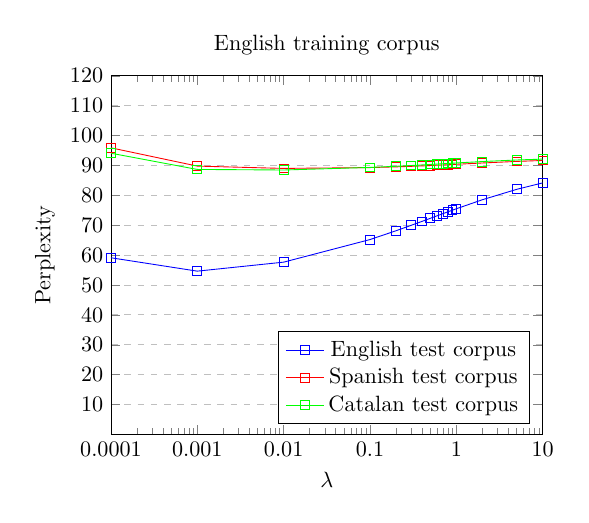
\begin{tikzpicture}[scale=.8]
\begin{semilogxaxis}[
	  log ticks with fixed point,
    title={English training corpus},
    xlabel={$\lambda$},
    ylabel={Perplexity},
    xmin=.0001, xmax=10,
    ymin=0, ymax=120,
    xtick={.0001,.001,.01,.1,1,10},
    ytick={10,20,30,40,50,60,70,80,90,100,110,120},
    legend pos=south east,
    ymajorgrids=true,
    grid style=dashed,
]
 
\addplot[
    color=blue,
    mark=square,
    ]
    coordinates {
(0.00010000,59.1283089317215982)
(0.00100000,54.6517234805657637)
(0.01000000,57.6610332070268115)
(0.10000000,65.2217161334261419)
(0.20000000,68.1635906438678205)
(0.30000000,69.9831803813590625)
(0.40000000,71.3026962861484179)
(0.50000000,72.3347625873169022)
(0.60000000,73.1792631974425802)
(0.70000000,73.8915354220917777)
(0.80000000,74.5055680064687351)
(0.90000000,75.0437767587365698)
(1.00000000,75.5217382188793209)
(2.00000000,78.5401805376036037)
(5.00000000,82.0240976713278229)
(10.00000000,84.1827238467045902)
    };

\addplot[
    color=red,
    mark=square,
    ]
    coordinates {
(0.00010000,95.9125002627099690)
(0.00100000,89.7961286097155948)
(0.01000000,89.0237350415562219)
(0.10000000,89.3062299111504103)
(0.20000000,89.5391996101755296)
(0.30000000,89.7177723781035326)
(0.40000000,89.8632630391371379)
(0.50000000,89.9858010250467970)
(0.60000000,90.0913250052520880)
(0.70000000,90.1836990724573582)
(0.80000000,90.2656028562934125)
(0.90000000,90.3389784351551555)
(1.00000000,90.4052806002390952)
(2.00000000,90.8430598534996392)
(5.00000000,91.3664112136055735)
(10.00000000,91.6813502239128297)
    };

\addplot[
    color=green,
    mark=square,
    ]
    coordinates {
(0.00010000,94.1046507794276152)
(0.00100000,88.6815928254827384)
(0.01000000,88.4936992000500453)
(0.10000000,89.3522510341229435)
(0.20000000,89.7382678865458701)
(0.30000000,89.9955260989669483)
(0.40000000,90.1904259540010429)
(0.50000000,90.3470560356094694)
(0.60000000,90.4774541960382379)
(0.70000000,90.5886622878672512)
(0.80000000,90.6852071296326017)
(0.90000000,90.7701885777525206)
(1.00000000,90.8458283478004063)
(2.00000000,91.3212440525163913)
(5.00000000,91.8434343417199130)
(10.00000000,92.1383844537980821)
    };
    \legend{English test corpus,Spanish test corpus,Catalan test corpus}
 
\end{semilogxaxis}
\end{tikzpicture}
\qquad
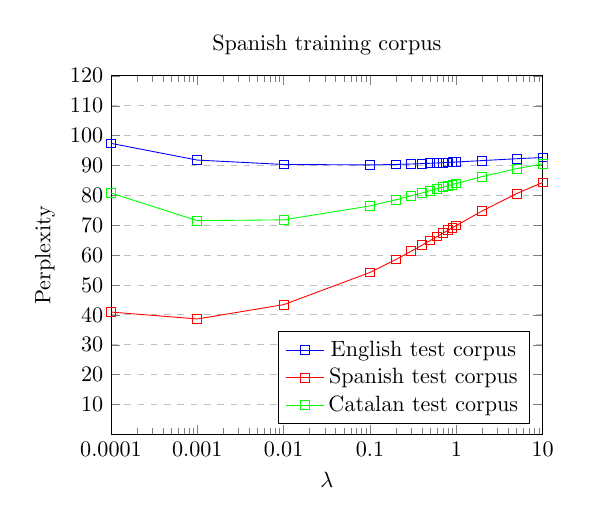
\begin{tikzpicture}[scale=.8]
\begin{semilogxaxis}[
	  log ticks with fixed point,
    title={Spanish training corpus},
    xlabel={$\lambda$},
    ylabel={Perplexity},
    xmin=.0001, xmax=10,
    ymin=0, ymax=120,
    xtick={.0001,.001,.01,.1,1,10},
    ytick={10,20,30,40,50,60,70,80,90,100,110,120},
    legend pos=south east,
    ymajorgrids=true,
    grid style=dashed,
]
 
\addplot[
    color=blue,
    mark=square,
    ]
    coordinates {
(0.00010000,97.4011888994087229)
(0.00100000,91.8113326669431586)
(0.01000000,90.3481014923758181)
(0.10000000,90.1910296056551601)
(0.20000000,90.3474557963722447)
(0.30000000,90.4975810808364827)
(0.40000000,90.6305084994941978)
(0.50000000,90.7476055741140328)
(0.60000000,90.8514097703866099)
(0.70000000,90.9441960143815038)
(0.80000000,91.0278085551387193)
(0.90000000,91.1037126289304666)
(1.00000000,91.1730737726991123)
(2.00000000,91.6488940732536150)
(5.00000000,92.2646209199521508)
(10.00000000,92.6712659443569038)
    };

\addplot[
    color=red,
    mark=square,
    ]
    coordinates {
(0.00010000,40.9639438998515004)
(0.00100000,38.6584153753228321)
(0.01000000,43.4415292344909076)
(0.10000000,54.2127005765265864)
(0.20000000,58.5692680167594588)
(0.30000000,61.3160844954069475)
(0.40000000,63.3332253349566443)
(0.50000000,64.9260564481858182)
(0.60000000,66.2395547276860839)
(0.70000000,67.3546940599671444)
(0.80000000,68.3215397850509021)
(0.90000000,69.1732970830234564)
(1.00000000,69.9331545756946582)
(2.00000000,74.8108793989151906)
(5.00000000,80.6206980976027552)
(10.00000000,84.3101043065777560)
    };

\addplot[
    color=green,
    mark=square,
    ]
    coordinates {
(0.00010000,80.7829345245770583)
(0.00100000,71.5528274889652209)
(0.01000000,71.8107081026033853)
(0.10000000,76.4706463647400909)
(0.20000000,78.5317674948841216)
(0.30000000,79.8503846726142399)
(0.40000000,80.8228044752091819)
(0.50000000,81.5911509778608774)
(0.60000000,82.2241320243881120)
(0.70000000,82.7605660652243529)
(0.80000000,83.2246406959750828)
(0.90000000,83.6324846758130462)
(1.00000000,83.9954043529956351)
(2.00000000,86.2967780687710331)
(5.00000000,88.9439727679360601)
(10.00000000,90.5526988538777005)
    };
    \legend{English test corpus,Spanish test corpus,Catalan test corpus}
 
\end{semilogxaxis}
\end{tikzpicture}

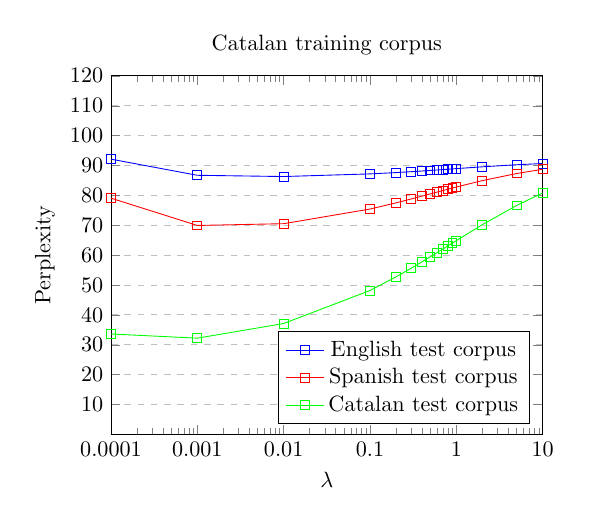
\begin{tikzpicture}[scale=.8]
\begin{semilogxaxis}[
	  log ticks with fixed point,
    title={Catalan training corpus},
    xlabel={$\lambda$},
    ylabel={Perplexity},
    xmin=.0001, xmax=10,
    ymin=0, ymax=120,
    xtick={.0001,.001,.01,.1,1,10},
    ytick={10,20,30,40,50,60,70,80,90,100,110,120},
    legend pos=south east,
    ymajorgrids=true,
    grid style=dashed,
]
 
\addplot[
    color=blue,
    mark=square,
    ]
    coordinates {
(0.00010000,92.1240701265360258)
(0.00100000,86.7242459209968075)
(0.01000000,86.3077754914684476)
(0.10000000,87.1903408517123353)
(0.20000000,87.6277188157458937)
(0.30000000,87.9276816442450837)
(0.40000000,88.1586557165922358)
(0.50000000,88.3464086947996634)
(0.60000000,88.5041310168937230)
(0.70000000,88.6396664007994559)
(0.80000000,88.7581167123006622)
(0.90000000,88.8630065781164831)
(1.00000000,88.9568797914650702)
(2.00000000,89.5594574975564655)
(5.00000000,90.2524660257874984)
(10.00000000,90.6602507930754911)
    };

\addplot[
    color=red,
    mark=square,
    ]
    coordinates {
(0.00010000,79.0766895724054990)
(0.00100000,69.9389145669934322)
(0.01000000,70.5322378695885419)
(0.10000000,75.4258936041369736)
(0.20000000,77.4968810265583983)
(0.30000000,78.8019379999643519)
(0.40000000,79.7549068495853675)
(0.50000000,80.5020333991339641)
(0.60000000,81.1134573261355740)
(0.70000000,81.6285916757146168)
(0.80000000,82.0718907384428178)
(0.90000000,82.4596023787350560)
(1.00000000,82.8030795142188367)
(2.00000000,84.9447909416295630)
(5.00000000,87.3226009360844841)
(10.00000000,88.7221523172377431)
    };

\addplot[
    color=green,
    mark=square,
    ]
    coordinates {
(0.00010000,33.6300430098770633)
(0.00100000,32.2281295519186131)
(0.01000000,37.1268291594521500)
(0.10000000,48.1674725711669325)
(0.20000000,52.7301967956830921)
(0.30000000,55.6316770632262276)
(0.40000000,57.7746847350702524)
(0.50000000,59.4744940549447492)
(0.60000000,60.8814196644865007)
(0.70000000,62.0796932293630093)
(0.80000000,63.1215385142198571)
(0.90000000,64.0416763035989050)
(1.00000000,64.8644065435427990)
(2.00000000,70.1905597353149346)
(5.00000000,76.6487554621150196)
(10.00000000,80.8246520215136002)
    };
    \legend{English test corpus,Spanish test corpus,Catalan test corpus}
 
\end{semilogxaxis}
\end{tikzpicture}

\end{center}